\protect \section *{\protect \nameref  *{WawesInLinearMedia}}
\begin{Solution}{8.{10}}
	$\alpha_{ik} = \frac{e^2}{m(\omega_0^2 - \omega^2)}\delta_{ik} - i \frac{e^3\omega H_{0l}}{m^2c(\omega_0^2 - \omega^2)^2}e_{ikl}$, $\vect{g} = -\frac{e^3\omega}{m^2c(\omega_0^2 - \omega^2)^2}\Hfield_0$
\end{Solution}
\begin{Solution}{8.{15}}
	$n = \sqrt{1 - \frac{\omega_p^2}{\omega^2}}$, де $\omega_p = \frac{4\pi N e^2}{n}$~---плазмова частота.
\end{Solution}
\begin{Solution}{8.{16}}
	\begin{equation*}
		\{ \epsilon \}  = \left( {\begin{array}{*{20}{c}}
				\alpha       & {i\beta } & 0      & \\
				{ - i\beta } & \alpha    & 0      & \\
				0            & 0         & \gamma &
			\end{array}} \right),
	\end{equation*}
	де константи $\alpha$, $\beta$, $\gamma$ задані формулами:
	\begin{align*}
		\alpha =  1 - \frac{\omega_p^2}{\omega ^2 - \omega _B^2},           \\
		\beta = \frac{\omega_B\omega_p^2}{\omega(\omega ^2 - \omega _B^2)}, \\
		\gamma = 1 - \frac{\omega _p^2}{\omega ^2},
	\end{align*}
	де $\omega _p^2 = \frac{4\pi n_e e^2}{m_e}$, $\omega_B = \frac{\left| e \right|B}{m_ec}$.
\end{Solution}
\begin{Solution}{8.{17}}
    Магнітне поле направимо по осі $OZ$ (в декартових координатах) та позначимо \(\vect{m}_{\pm} = (1, \mp i,0)\), \(k_\pm^2 = \frac{\omega }{c^2} \cdot \frac{\omega^2 \pm \omega \omega_B - \omega_p^2}{\omega  \pm \omega_B}\).

    Для хвиль, що поширюються у додатному напрямку осі $OZ$, розв’язки рівнянь Максвелла мають вигляд $\Efield = E_0\vect{m}_{\pm} e^{i(k_\pm z - \omega t)}$ при $\omega > 0$ для дійсного $k_{\pm} >0$.

    Хвилі з поляризацією $\vect{m}_+$ проходять у додатному напрямку осі $OZ$ при \(\omega  > \omega_1 = \sqrt {\frac{{\omega_B^2}}{4} + \omega_p^2}  - \frac{\omega _B}{2}\).

    Хвилі з поляризацією $\vect{m}_-$ проходять при \(0<\omega<\omega_B\)  та при\\\(\omega  > \sqrt {\frac{\omega_B^2}{4} + \omega_p^2}  + \frac{\omega _B}{2}\).

    Якщо \({\omega _p} > \sqrt 2 {\omega _B}\), тоді  інтервал \(\omega_B  <  \omega_1 \)  є забороненим для обох типів хвиль.
\end{Solution}
\begin{Solution}{8.{18}}
    Виберемо вісь $OZ$ декартових координат у напрямку руху хвилі, електричне поле направимо по осі OX. Шукаємо розв’язок у вигляді:
    \begin{align*}
        \Efield &= E_1\vect{e}_x e^{i(k_1z - \omega t)}, \quad z<0, \\
        \Efield &= E_2\vect{e}_x e^{i(k_2z + \omega t)} + E'_2\vect{e}_x e^{-i(k_2z + \omega t)}, \quad 0<z<d, \\
        \Efield &= E_2\vect{e}_x e^{i(k_2(z-d) - \omega t)}, \quad z>d,
    \end{align*}
    де $k_s = \frac{\omega_s}{c}n_s$, $s = 1,2,3$.

    Магнітні поля отримуємо з рівнянь Максвелла. З граничних умов для тангенціальних компонент електричного та магнітного поля при $z = 0$ маємо:
    \[
        E_2 = \frac{1}{2}\left(1 + \frac{k_1}{k_2} \right){E_1}, \quad E'_2 = \frac{1}{2}\left( 1 - \frac{k_1}{k_2} \right){E_1}.
    \]

    З граничних умов при  $z = d$:
    \[
        e^{ik_2d}{E_2} = \frac{1}{2}\left( 1 + \frac{k_3}{k_2} \right)E_3, \quad E'_2e^{- ik_2d} = \frac{1}{2}\left( 1 - \frac{k_3}{k_2} \right)E_3.
    \]
    Аналіз сумісності цих рівнянь дає умову існування нетривіального розв’язку:
    \[
        e^{2ik_2d} = \frac{(n_2 - n_1)(n_2 + n_3)}{(n_2 + n_1)(n_2 - n_3)}.
    \]
    Ліва частина цього співвідношення є дійсною, коли вона дорівнює $1$ чи $-1$. Звідси маємо дві можливості:
    \begin{equation*}
    d=
    \begin{cases}
    m\frac{\lambda_2}{2}, \quad n_1 = n_3\\
    (2m+1)\frac{\lambda_2}{2}, \quad n_2^2 = n_1n_3
    \end{cases}.
    \end{equation*}
    де $\lambda_2 = \frac{2\pi c}{\omega n_2}$.
\end{Solution}
\begin{Solution}{8.{20}}
	На рисунку показана плоска хвиля, яка поширюється в напрямку $x$ перпендикулярно до металевого циліндра, вісь якого напрямлена вздовж осі $z$.

	\begin{center}
		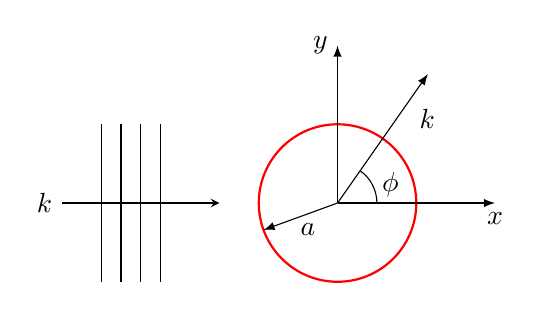
\begin{tikzpicture}
			\draw[red, thick] (0,0) circle (1);
			\draw[-latex] (0,0) -- ++(2,0) node[below] {$x$};
			\draw[-latex] (0,0) -- ++(0,2) node[left] {$y$};
			\draw[-latex] (0,0) -- node[pos=0.8, anchor=north west] {$\vect{k}$} (55:2);
			\draw (0,0) ++(0:0.5) arc (0:55:0.5) node[anchor=west, pos=0.5] {$\phi$};
			\draw[-latex] (0,0) -- node[below, pos=0.4] {$a$} ++(200:1);
			\draw foreach \i in {-3,-2.75,-2.5,-2.25} {(\i,1) -- (\i,-1) };
			\draw[-stealth] (-3.5, 0) node[left] {$\vect{k}$} -- ++(2,0);
		\end{tikzpicture}
		\captionof{figure}{До пояснення задачі}
	\end{center}

    Розглянемо випадок а) ($\Efield \parallel \vect{e}_z$).

	Поляризація, паралельна до осі циліндра, викликає поверхневі струми лише у напрямку осі $z$, а тому магнітного поля вздовж осі $z$ немає.
%     $B_z = (\rot{\vect{A}})_z = 0$. З іншого боку $E_z = -\partial_z\pot - \partial_t A_z \neq 0$, таким чином, звідси випливає, що поза циліндром:
%	\[
%		B_{\phi} = -E_z.
%	\]
%
%	Поляризація, перпендикулярна до осі циліндра індукує поверхневі струми в напрямку $\vect{e}_{\phi}$, тому магнітне поле напрямлене вздовж осі $z$, а відповідно електричне поле поза межами циліндра (область хвиль) визначається як:
%	\[
%		B_z = E_{\phi}.
%	\]

	Монохроматична плоска хвиля з частотою $\omega$ індукує  гармонічні струми і, як наслідок ми маємо розсіяну хвилю, яка теж є гармонічною.

	Поза циліндром електричне та магнітне поля задовольняють хвильовому рівнянню.
	Тому просторові частини $E_z$ і $B_z$ задовольняють рівнянню Гельмгольца:
	\[
		\left[ \Delta + \frac{\omega^2}{c^2}\right] u = 0,
	\]
	або в циліндричних координатах:
	\[
		\frac1r \frac{\partial }{\partial r}
		\left( r \frac{\partial u}{\partial r} \right) + \frac{1}{r^2} \frac{\partial^2 u}{\partial \phi^2} + k^2 u = 0.
	\]

	Розділимо змінні в останньому рівнянні $u(r,\phi) = R(r)G(\phi)$, одразу отримаємо $G(\phi) = e^{\pm im\phi}$, а рівняння для $R(r)$, як відомо, задовольняє рівняння диференціальному Бесселя~\eqref{eq:Bessel_eq}, якщо покласти $x = kr$:

\begin{equation}\label{eq:BessProblem}\tag{*}
		\frac{d^2R}{dx^2} + \frac1x\frac{dR}{dx} + \left(1 - \frac{m^2}{x^2} \right) R = 0,
\end{equation}

	розв'язок якого, як відомо, можна представити за допомогою функцій Бесселя $J_m(x)$ та Неймана $N_m$.
%    Однак, оскільки для нашої задачі розсіяна хвиля має бути циліндричною при $r \to\infty$, тому
    В нашому випадку краще скористатись функціями Ганкеля 1-го роду, що дають асимптотику на нескінченності $e^{ikr}/\sqrt{r}$ (див.~\eqref{eq:Hxgg1}), яка відповідає умовам випромінювання.

    Поле  $E_z$ розсіяної хвилі будемо шукати як  лінійну комбінацію функцій $H_m^{(1)}e^{im\phi}$ з коефіцієнтами $A_m$:
	\[
		E_{z,\text{розс}} =  \sum\limits_{m = -\infty}^{\infty} A^m H^{(1)}_m(k r)e^{im\phi}.
	\]

	Поле плоскої падаючої хвилі $ E_{z,\text{пад}} = E_0e^{ikx} = E_0e^{ikr\cos\phi}$ розкладемо за функціями Бесселя (див~\eqref{eq:JacobiAnger}):
	\[
		E_{z,\text{пад}} =  E_0e^{ikr\cos\phi} =  E_0 \sum\limits_{m = -\infty}^{\infty} i^m J_m(k r)e^{im\phi}.
	\]

	Загальне поле є сумою падаючої та розсіяної хвиль, за принципом суперпозиції:
	\[
		E_z = E_0 \sum\limits_{m = -\infty}^{\infty}[ i^mJ_m(kr) + A_mH^{(1)}_m(kr)]e^{im\phi}.
	\]

	Далі скористаємось граничною умовою $E_z(r = a) = 0$  і визначимо $a_m$ з рівняння~\eqref{eq:BessProblem}; матимемо:
	\[
		E_z(r,\phi) = E_0e^{ikr\cos\phi} - E_0\sum\limits_{m = -\infty}^{\infty} i^m \frac{J_m(ka)}{H_m^{(1)}(ka)}H_m^{(1)}(kr)e^{im\phi}.
	\]

    Магнітне поле отримуємо з рівняння Максвелла $\Bfield = \frac1k\rot\Efield = \frac1k \vect{\nabla}E_z\times \vect{e}_z$,

    \[
        B_r=\frac{1}{kr}\frac{\partial E_z}{\partial \phi},
    \]
    \[
        B_\phi=-\frac{1}{k}\frac{\partial E_z}{\partial r}.
    \]

    Легко  перевірити, що $B_r=0$ при $r=a$ на  поверхні надпровідного циліндра і, таким чином, задовольняє граничній умові.

    Випадок б) ($\Efield \perp \vect{e}_z$).

	Для перпендикулярної поляризації викладки аналогічні, але тут зручніше починати з складової магнітного поля, яке у плоскій хвилі має вигляд $B_z = E_0e^{ikx}$. Гранична умова для тангенціальної компоненти електричного поля дає:
	\[
		E_{\phi}(r = a) = \left. \frac1k\frac{\partial B_z}{\partial r}\right|_{r = a} = 0.
	\]

	Отже
	\[
		B_z = E_0e^{ikr\cos\phi} - E_0\sum\limits_{m = -\infty}^{\infty} i^m \frac{J_m'(ka)}{H_m^{(1)\prime}(ka)}H_m^{(1)}(kr)e^{im\phi},
	\]
	де штрих <<$\prime$>> означає похідну по радіальній аргументу $kr$.

	Знайдемо тепер диференціальні перерізи розсіювання
	\(
	\frac{d\sigma}{d\phi} = r \frac{|\Efield_\text{розс}|^2}{|\Efield_\text{пад}|^2}
	\).

	Враховуючи, що$\lim\limits_{r\to\infty}H_m^{(1)}(kr) = \sqrt{\frac{2}{\pi k r}}$, маємо:
	\[
		\frac{d\sigma_{\parallel}}{d\phi} = \frac{2}{\pi k} \left| \sum\limits_{m = -\infty}^{\infty} \frac{J_m(ka)}{H_m^{(1)}(ka)}e^{im\phi} \right|^2, \quad
		\frac{d\sigma_{\perp}}{d\phi} = \frac{2}{\pi k} \left| \sum\limits_{m = -\infty}^{\infty} \frac{J_m(ka)'}{H_m^{(1)\prime}(ka)}e^{im\phi} \right|^2.
	\]

	Ці диференціальні перерізи мають розмірність довжини (а не площі), оскільки вони визначають потужність на одиницю довжини циліндра, тобто потужність, випромінювана через границю великого кола, співвісного з циліндром.

	Повні перерізи:
	\[
		\sigma_{\parallel} = \frac4k \sum\limits_{m = -\infty}^{\infty} \frac{J_m^2(ka)}{J_m^2(ka) + N_m^2(ka)}, \quad
		\sigma_{\perp} = \frac4k \sum\limits_{m = -\infty}^{\infty} \frac{J_m^{2\prime}(ka)}{J_m^{2\prime}(ka) + N_m^{2\prime}(ka)}.
	\]
\end{Solution}
\begin{Solution}{8.{21}}
На рисунку показана плоска хвиля, яка поширюється в напрямку $x$ перпендикулярно до діелектричного циліндра, вісь якого напрямлена вздовж осі $z$.

	\begin{center}
		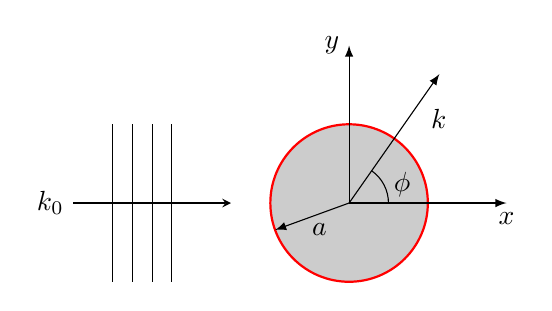
\begin{tikzpicture}
			\draw[red, thick, fill=gray!40] (0,0) circle (1);
			\draw[-latex] (0,0) -- ++(2,0) node[below] {$x$};
			\draw[-latex] (0,0) -- ++(0,2) node[left] {$y$};
			\draw[-latex] (0,0) -- node[pos=0.8, anchor=north west] {$\vect{k}$} (55:2);
			\draw (0,0) ++(0:0.5) arc (0:55:0.5) node[anchor=west, pos=0.5] {$\phi$};
			\draw[-latex] (0,0) -- node[below, pos=0.4] {$a$} ++(200:1);
			\draw foreach \i in {-3,-2.75,-2.5,-2.25} {(\i,1) -- (\i,-1) };
			\draw[-stealth] (-3.5, 0) node[left] {$\vect{k}_0$} -- ++(2,0);
		\end{tikzpicture}
		\captionof{figure}{До пояснення задачі}
	\end{center}

	Вказівка: дивіться розв'язок задачі~\ref{prb:Zang_metall_Cyllinder} і врахуйте необхідну поляризацію, та граничні умови для поля на межі розділу.

	Поле в циліндрі $r < a$ шукаємо у вигляді:
	\[
		E_{z,\text{in}} = \sum\limits_{m = -\infty}^{\infty}A_mJ_m(kr)e^{im\phi}, \quad k=\sqrt{\epsilon} \omega/c.
	\]

	Зовні, електричне поле є сумою падаючої та розсіяної хвилі:
	\[
		E_z = E_0 \sum\limits_{m = -\infty}^{\infty} \left( i^m J_m(k_0 r) + B_m H_m^{(1)(k_0r)} \right) e^{im\phi}, \quad k= \omega/c.
	\]
	де
	\[
		A_m = E_0i^m \frac{  H_m^{(1)}(k_0a) J'_m(k_0a) - H_m^{(1)\prime}(k_0a) J_m(k_0a)    }{ \sqrt{\epsilon} H_m^{(1)}(k_0a) J'_m(ka) - H_m^{(1)\prime}(k_0a) J_m(ka)},
	\]
	\[
		B_m = E_0i^m \frac{  J_m(ka) J'_m(k_0a) - \sqrt{\epsilon} J_m'(ka) J_m(k_0a)    }{ \sqrt{\epsilon} H_m^{(1)}(k_0a) J'_m(ka) - H_m^{(1)\prime}(k_0a) J_m(ka)}.
	\]

\end{Solution}
\begin{Solution}{8.{22}}
    За умови задачі  електричне і магнітне поля хвилі, які можна вважати квазистаціонарними, індукують в надпровідній кулі електричний дипольний момент $p_e=ER^3$ та магнітний момент $p_m=-BR^{3/2}$. Звідси отримуємо сумарне магнітне поле в хвильовій зоні за формулами дипольного та магнітодипольного випромінювання.
	Диференціальний переріз
	\[
		\frac{d\sigma}{do} = R^6 k^4 \left[\frac58 (1 + \cos^2\theta) -\cos\theta\right],
	\]
	де $k$~--- хвильове число, $\theta = \widehat{\vect{k}_0,\vect{k}}$~--- кут між напрямками падаючої та розсіяної хвилі.
	Повний переріз $\sigma = \frac{10\pi R^6 k^4}{3}$.
\end{Solution}
\begin{Solution}{8.{23}}
	$I(x,y) = I_0\frac{\sin^2\alpha}{\alpha^2}\frac{\sin^2\beta}{\beta^2}$, де $\alpha = \frac{kax}{2l}$, $\beta=\frac{kby}{2l}$.
\end{Solution}
\begin{Solution}{8.{24}}
    Вказівка: при інтегруванні слід врахувати співвідношення для функцій Бесселя~\eqref{eq:recInt} $\int\limits_0^x x'J_0(x')dx' = xJ_1(x)$.

	Відповідь: $I(r) = 4I_0\left( \frac{J_1\left( \frac{kRr}{l}\right) }{\frac{kRr}{l}}\right)^2$.
\end{Solution}
